\begin{frame}{broadcast/multicast}
\begin{itemize}
\item UDP IPv4: can broadcast to every machine on local network
    \begin{itemize}
    \item set the SO\_BROADCAST socket option to 1
    \item send to special address 255.255.255.255 
    \item received at that port number on all machines
    \end{itemize}
\item UDP multicast: (send-to-many) groups
    \begin{itemize}
    \item to receive: IP\_ADD\_MEMBERSHIP (v4), IPV6\_ADD\_MEMBERSHIP (v6)
        \begin{itemize}
        \item via setsockopt
        \end{itemize}
    \item each `multicast group' has IP address
    \item 224.0.0.0/24 and ff02::/16 = local network only
    \item local network: can implement by broadcasting + filtering
    \item (non-local-network multicast is more complex\ldots)
    \end{itemize}
\end{itemize}
\end{frame}

\begin{frame}{service discovery}
\begin{itemize}
\item example: find printers on local network automatically
\vspace{.5cm}
\item typical protocol mDNS (`multicast DNS')
\item uses IP addressses 224.0.0.251 / ff02::fb + port 5353
\item all machines on local network receive from all other machines on local network
\end{itemize}
\end{frame}

\begin{frame}[fragile]{multicast DNS request}
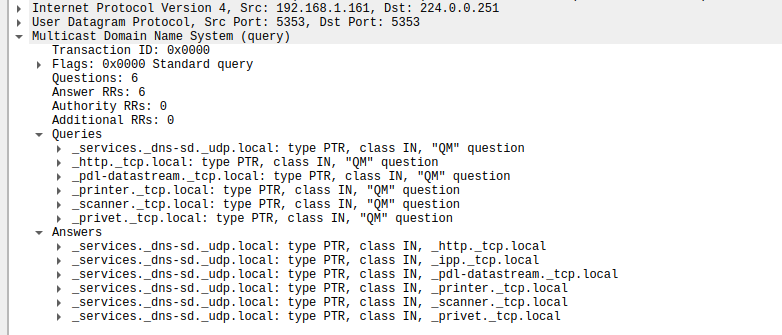
\includegraphics[height=0.85\textheight]{../sockets/mdns-request}
\end{frame}

\begin{frame}[fragile]{multicast DNS response}
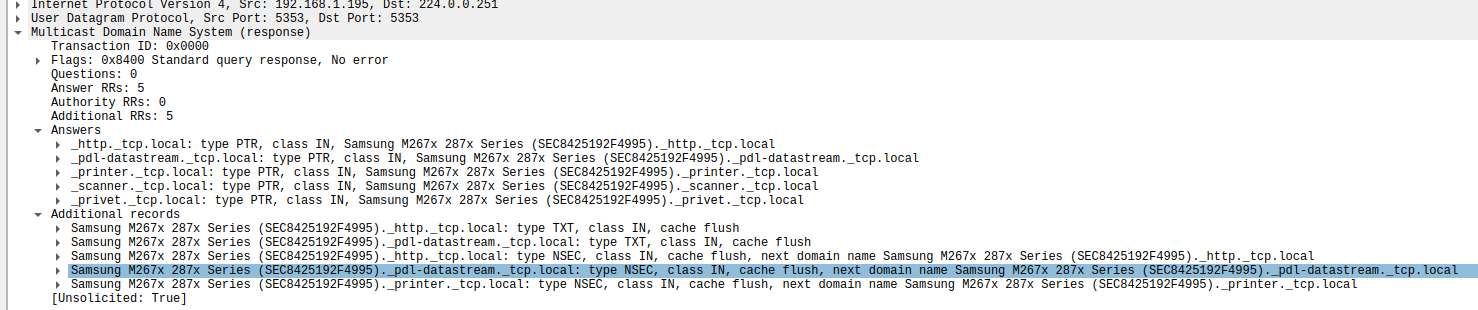
\includegraphics[height=0.85\textheight]{../sockets/mdns-response}
\end{frame}

\begin{frame}{.local domain}
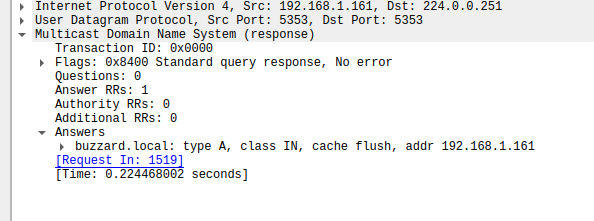
\includegraphics[height=0.85\textheight]{../sockets/unsolict-local-mdns}
\end{frame}
